We have evaluated two main areas;
\begin{itemize}
	\item The functional solidity --- using log files and JUnit~\cite{junit} tests
	\item The front-end usability --- using the Think Aloud Protocol
\end{itemize}

Clearly, both areas are important for a successful software system. 

\section{Functional Solidity}\label{policy-engine-system-evaluation}
JUnit tests are structured, assertable software tests that ensures that the software behaves as expected. Of course TDD\footnote{Test Driven Development} --- which we employed using the development of the core functionality --- has it's limits, mainly with regards to the quality of the written tests. The JUnit test accounts for the low level implementation tests.

On a higher abstraction level, we employ log files for testing. A log file is being generated at run-time, and has been integrated into (amongst other areas) the expression language. An example; we already know a certain policy's expected behavior (because we defined it ourselves) --- then we make sure that the policy is executed by the policy engine, and after the successful execution we carefully study the log file and compare it with the expected behavior. We find the log tests a natural selection on top of the more low level automated JUnit tests. It gave us a sense of extra security in regards to the behavior of the policy engine.

\subsection{Log Testing}
\label{log-test}
We have logged system data which was important as to determine if the system was working correctly. Doing so we have been able to verify the behavioral results and to discover bugs in our implementation --- which we then iteratively corrected. 

We have also been using the log files for source code quality control. We verified our solution by cross-referencing every action during tests, and matched it with the actual data stored in the database.

One excerpt from the log file can be seen in figure \ref{fig:log}

\begin{figure}[ht]
\centering
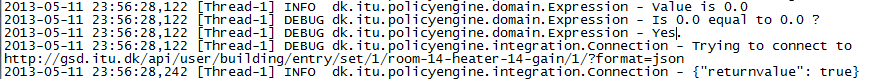
\includegraphics[width=\columnwidth]{images/logoutput.png}
\caption{An excerpt from the log file.}
\label{fig:log}
\end{figure}

\subsection{JUnit Testing}
To strengthen the solidity of the software, and minimize time used on debugging, we implemented a suite of JUnit Tests. An snippet of JUnit code can be seen in \ref{fig:junit-example}. Entering this test, the \textit{ROOM1\_HEATER} has been set to 1 and \textit{ROOM1\_TEMPERATURE} has been set to 26. The purpose is to see if the underlying expression language will set the \textit{ROOM1\_HEATER} to 0, which it should because the Expression's condition is using the \textit{Operator.GREATER\_THAN} along with a value of 25.
 
We have employed a sufficient amount of JUnit tests, to test all operators and both IfStatements (including nested capabilities) and SetStatements.

The result was that our IF-THEN-ELSE concept implementation performed as expected.

\begin{figure}[ht]
\centering
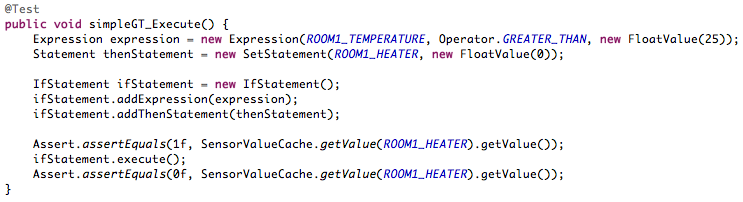
\includegraphics[scale=.5]{images/appendix-junit-example.png}
\caption{A snippet of a JUnit test.}
\label{fig:junit-example}
\end{figure}

\section{Usability Test}\label{sec:usability-test}
By using the Think Aloud Protocol we tested to uncover potential usability issues that needed solving.

To evaluate on the usability of our policy engine we decided to make a test with participants outside of our development group. In general, when it comes to "best practices of usability tests", the Think Aloud Protocol is considered one of the most valuable \cite{Nielsen1993}.

The Think Aloud Protocol is time wise inexpensive and easy to set up and it also gives very valuable result from real-life scenarios.

\subsection{Think Aloud Protocol}
In a Think Aloud Test, you ask test participants (one at a time) to use the system while continuously thinking out loud --- that is  simply verbalizing their thoughts as they move through the user interface, and take actions.

To run a basic Think Aloud usability study, three things are required:

\begin{itemize}
\item Recruit representative participants.
\item Inform them of representative tasks to perform.
\item Avoid interference and let the participants speak their actions.
\end{itemize}

We invited five people to each Think Aloud Test. Research shows that having just five people will potentially uncover 80\% of all usability problems \cite{jakobnielsen2000fiveusers} as seen on \ref{fig:usabilitycurve}.

We conducted two Think Aloud Tests, these tests were aimed at fixing any usability issues found during the third iteration.

\begin{figure}[ht]
\centering
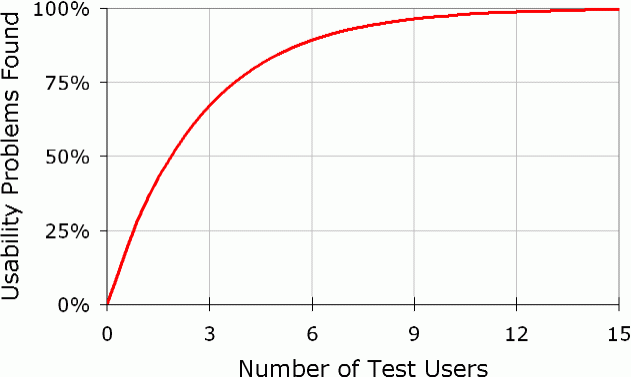
\includegraphics[width=\columnwidth]{usabilitycurve.png}
\caption{Usability test graph.}
\label{fig:usabilitycurve}
\end{figure}

We have not directly targeted Facility Managers in our usability tests, as we simply did not have the time to gather enough test persons with a relevant job function. However instead we gathered a broad range of random test persons with different backgrounds and age.

\subsubsection{Tasks}
We arranged 10 tasks for the participants to perform. Note however that the tests where held individually, but they were all given the same set of tasks. 
During the tests, participants where only given one task at a time to focus on - using small task cards.

Before the test started we explained the purpose of the policy engine, and verbally gave them an example of a user scenario.

We briefly introduced the participant to a map of the building and the rooms involved. We also gave an example list of sensor and actuator names to make them familiar with the elements involved, including basic knowledge of IF, AND, THEN statements and wildcard operators. The questions were designed so that the test persons used all of the features available in the policy engine. The user interface contain an \textit{live auto-complete function} so that the participant can easily set a desired sensor/actuator without knowing the exact name. See section \ref{managing-policies} for more details.

The participants where assigned the following tasks:

\begin{framed}
Create a policy that turns the AC on in Room 1, 1. floor and name it "Cooling".
\end{framed}
The 1st task was designed to see how the participant would try to create new policies - and how they would set the name.

\begin{framed}
Modify the "Cooling" policy just created to affect both Room 1, 1. floor and Room 2, 2. floor.
\end{framed}
The 2nd task was designed to see how the participant handled modifying an existing policy.

\begin{framed}
Create a policy that turns on blinds in all rooms for every floor in the building and name the policy "Sun".
\end{framed}
The 3rd task was designed to see how the participant handled the "wildcard" auto-complete feature.

\begin{framed}
Find and show the active policies just created.
\end{framed}
This 4th task showed how well the participant handled the listing of active policies --- as this would likely be a typical reoccurring task for a building administrator.

\begin{framed}
Disable the policy named "Cooling" so that it is no longer in function.
\end{framed}
The 5th task showed how well the participant handled enabling/disabling of a policy.

\begin{framed}
Delete the policy named "Sun".
\end{framed}
The 6th task showed the removal of policies.

The tasks 7-10 were designed to be harder and the participant was forced to work with complex expressions.

\begin{framed}
To save energy the university wants to have the heating turned OFF automatically at 17:00. However this Wednesday around 19:00 - 22:00 an exclusive presentation is held in room number 5 on 1. floor.
You are asked to maintain a temperature at 21 degrees in that room throughout the presentation.
\end{framed}

\begin{framed}
It is summertime and the overall temperature inside the building is rising. You are asked to keep the temperature at maximum 22 in all of the rooms in the building.
\end{framed}

\begin{framed}
All afternoon between 12:00 and 16:00 the sun is at its peak. Therefore you are asked to set blinds ON in all the rooms on 1. floor and 2. floor - but only if the lights are ON.
\end{framed}

\begin{framed}
The university wants to save energy. You are asked to make sure lights are automatic turned OFF at 17:00 in all the rooms, except from those on 0. Floor.
\end{framed}

\subsubsection{Results and Comments}
\label{results-and-comments}
After every participant had gone through the Think Aloud Test. We went through all their "thoughts" and issues. Some were the same, these we combined into one.
For all the remarks, we made some comments as listed below --- including the actions we took to further improve the software.

\begin{quotation}
If there is a lot of statements - which I would expect there will be? Then I think the statement list would be too long. I think it would make it difficult to keep the overview, if say you have 100 statements.
\end{quotation}

The participant were referring to the “detail view” of a policy, from which every statement were listed underneath each other. 

Due to this remark we have implemented an expand function, which instead of listing all the content at once, it now only shows each statement headline as an open / closable area.
 
\begin{quotation}
I think it is difficult to see which one (rule) belong to what (expression).
\end{quotation}

The participant were referring to the setup within a given policy. When a policy contains an IfStatement, the list of conditional expressions, and the then-clause and else-clause created some confusion. The participant found that it was difficult to separate the different parts.

Due to this we implemented the aforementioned color coding \ref{colorcodinglabel}.

In the second Think Aloud Test with five new persons, the result showed that they found the overview better and easier to understand after implementing this encapsulation and color coding.

After the second round of testing we only had some minor changes to do. But overall the participant where comfortable with the usability and had no further remarks.

We believe that there is always room for improvement, and we elaborate on this in the section \ref{subsec:improvements}.